\documentclass[conference]{IEEEtran}
\IEEEoverridecommandlockouts
\usepackage{cite}
\usepackage{amsmath,amssymb}
\usepackage{graphicx}
\usepackage{booktabs}
\usepackage{url}
\usepackage{xcolor}

% Placeholders (PH of a key) are replaced by scripts/fill_tex.py from results/*.json.
% The definition lets the unfilled source still compile (shows the key in red).
\newcommand{\PH}[1]{\textcolor{red}{\texttt{#1}}}

\begin{document}

\title{Knowing When to Abstain: Calibration and Selective Prediction\\
for Machine-Learning Network Intrusion Detection}

\author{\IEEEauthorblockN{Author One, Author Two}
\IEEEauthorblockA{Department / Affiliation \\ City, Country \\ \{a1, a2\}@example.edu}}

\maketitle

\begin{abstract}
Machine-learning intrusion detectors are routinely deployed with a single hard decision and no
notion of when their output should be trusted. We show, on the public NSL-KDD benchmark, that three
standard detectors (logistic regression, a random forest, and gradient boosting) are markedly
over-confident: expected calibration error reaches \PH{logreg_ece_raw}, and the strongest model still
attains an error rate of \PH{histgb_risk_full} on a test set whose attack mix it was trained on. We
then study two remedies. First, post-hoc Platt scaling fitted on in-distribution data fails to repair
calibration once the test distribution shifts, leaving error essentially unchanged. Second, selective
prediction---allowing the detector to abstain on its least-confident inputs---reduces selective risk
from \PH{histgb_risk_full} to \PH{histgb_risk80} at \mbox{80\%} coverage, but only for models whose
confidence is informative; logistic regression's confidence is nearly useless for ranking errors
(area under the risk--coverage curve \PH{logreg_aurc} versus \PH{histgb_aurc}). Finally, using a
controlled family-holdout protocol we quantify behaviour on \emph{unknown} attacks: detection of a
held-out family collapses (e.g.\ DoS from \PH{det_seen_DoS} to \PH{det_unseen_DoS}), and abstention
rejects only part of these unknowns---and almost none when the attack mimics benign traffic (R2L). We
conclude that selective prediction is a cheap, model-agnostic safety layer for ML intrusion detection,
with clearly characterised limits.
\end{abstract}

\begin{IEEEkeywords}
intrusion detection, selective prediction, calibration, uncertainty, open-set recognition, NSL-KDD
\end{IEEEkeywords}

\section{Introduction}
A network intrusion detector that emits only ``attack'' or ``benign'' gives an operator no way to tell
a confident verdict from a guess. In practice this matters twice over: alerts compete for scarce
analyst attention, and genuinely novel attacks---absent from any training corpus---are exactly the
cases a static classifier is least equipped to label. A detector that could say ``I am not sure'' on
these inputs, and defer them to a human or a secondary control, would be more useful than one forced
to commit.

This paper asks a narrow, practical question: do off-the-shelf machine-learning intrusion detectors
produce confidence scores that are trustworthy enough to drive such an abstention policy, and what do
they do when faced with attacks they have never seen? We answer empirically on NSL-KDD
\cite{tavallaee2009nsl}, a public benchmark whose published test split deliberately contains attack
types absent from training. Our contributions are:
\begin{itemize}
\item We measure the calibration of three standard detectors and show all are over-confident
(Section~\ref{sec:cal}), and that post-hoc Platt scaling \cite{platt1999probabilistic} fitted on
in-distribution data does \emph{not} transfer to the shifted test set.
\item We evaluate selective prediction \cite{elyaniv2010selective,geifman2017selective} and show
abstention cuts selective risk substantially, but that its usefulness is model-dependent: tree
ensembles rank their errors well, a linear model does not (Section~\ref{sec:sp}).
\item We introduce a controlled family-holdout protocol for the \emph{unknown-attack} regime and show
detection collapses on held-out families while abstention provides only partial cover---and almost
none for attacks that resemble benign traffic (Section~\ref{sec:openset}).
\end{itemize}
Throughout we follow the evaluation guidance of Arp \emph{et al.}\ \cite{arp2022dodos}: the calibrator
is fit only on held-out training data, and no test information leaks into model selection.

\section{Related Work}
\textbf{Calibration.} Modern classifiers often output probabilities that do not match empirical
accuracy \cite{guo2017calibration,niculescu2005predicting}. Expected calibration error (ECE) summarises
this gap, and temperature/Platt scaling are common post-hoc fixes \cite{platt1999probabilistic}. These
analyses typically assume the evaluation data is drawn from the training distribution---an assumption
that fails for intrusion detection.

\textbf{Selective prediction.} A classifier with a reject option \cite{elyaniv2010selective} trades
coverage for accuracy on what it does accept; the risk--coverage curve and its area
\cite{geifman2017selective} quantify the trade-off. Maximum softmax/posterior probability is a strong
baseline confidence score \cite{hendrycks2017baseline}.

\textbf{ML for intrusion detection.} The limits of learned detectors---especially on novel attacks and
under distribution shift---were argued early \cite{sommer2010outside} and remain a methodological
hazard \cite{arp2022dodos}. We do not propose a new detector; we ask whether existing ones know when
they are wrong.

\section{Methodology}
\textbf{Data.} NSL-KDD \cite{tavallaee2009nsl} provides \PH{n_train} training and \PH{n_test} test
records with 41 features (three categorical) and a binary normal/attack label; each attack maps to one
of four families (DoS, Probe, R2L, U2R). Its test split contains \PH{n_novel_types} attack \emph{types}
(\PH{n_novel_rows} records) that never appear in training---a built-in open-set test. Numeric features
are standardised and categorical features one-hot encoded; the encoder is fit on training data only.

\textbf{Models.} We use scikit-learn \cite{pedregosa2011scikit} logistic regression, a random forest,
and histogram gradient boosting---deliberately standard detectors, since our subject is their
confidence, not their architecture.

\textbf{Calibration.} For each model we report ECE (15 equal-width bins of the predicted class
probability) before and after Platt scaling, the latter fitted on a 20\% held-out split of the
training set.

\textbf{Selective prediction.} The confidence of a prediction is its maximum class probability. Sorting
the test set by confidence and accepting the most-confident fraction $c$ yields the selective risk
$r(c)$; we report the area under $r(c)$ (AURC) and $r(0.8)$.

\textbf{Open-set protocol.} To probe genuinely unknown attacks under control, we remove one attack
family entirely from training (keeping benign traffic and the other families), retrain, and measure
detection and confidence on that family's test records. We also report, at a global threshold giving
80\% coverage, the fraction of unknown-family records that abstention rejects.

\section{Results}
\subsection{Detectors are over-confident}\label{sec:cal}
Table~\ref{tab:main} reports accuracy and calibration. All three models are over-confident: ECE ranges
from \PH{rf_ece_raw} (random forest) to \PH{logreg_ece_raw} (logistic regression). Platt scaling, fit
on in-distribution held-out data, does not help on the shifted test set---ECE is essentially unchanged
for gradient boosting (\PH{histgb_ece_raw} to \PH{histgb_ece_cal}) and slightly worse for the random
forest (\PH{rf_ece_raw} to \PH{rf_ece_cal}). Calibrating to the source distribution does not certify
probabilities once the deployed distribution moves, as Fig.~\ref{fig:rel} illustrates.

\begin{table}[t]
\centering
\caption{Accuracy, calibration error (raw / after Platt scaling), and selective-prediction quality on
the NSL-KDD test set. Lower ECE and AURC are better.}
\label{tab:main}
\begin{tabular}{lccccc}
\toprule
Model & Acc. & ECE$_\text{raw}$ & ECE$_\text{Platt}$ & AURC & $r(0.8)$ \\
\midrule
Logistic reg.   & \PH{logreg_acc} & \PH{logreg_ece_raw} & \PH{logreg_ece_cal} & \PH{logreg_aurc} & \PH{logreg_risk80} \\
Random forest   & \PH{rf_acc}     & \PH{rf_ece_raw}     & \PH{rf_ece_cal}     & \PH{rf_aurc}     & \PH{rf_risk80} \\
Hist.\ grad.\ boost. & \PH{histgb_acc} & \PH{histgb_ece_raw} & \PH{histgb_ece_cal} & \PH{histgb_aurc} & \PH{histgb_risk80} \\
\bottomrule
\end{tabular}
\end{table}

\subsection{Abstention helps---if confidence is informative}\label{sec:sp}
Fig.~\ref{fig:rc} shows risk--coverage curves. For gradient boosting, abstaining on the least-confident
20\% of inputs lowers selective risk from \PH{histgb_risk_full} to \PH{histgb_risk80}; the random forest
behaves similarly (AURC \PH{rf_aurc}). Logistic regression is the cautionary case: its confidence
barely ranks its errors (AURC \PH{logreg_aurc}), so abstention buys little (\PH{logreg_risk_full} to
\PH{logreg_risk80}). The lesson is that selective prediction is only as good as the underlying
confidence signal, which here depends strongly on the model family.

\begin{figure}[t]
\centering
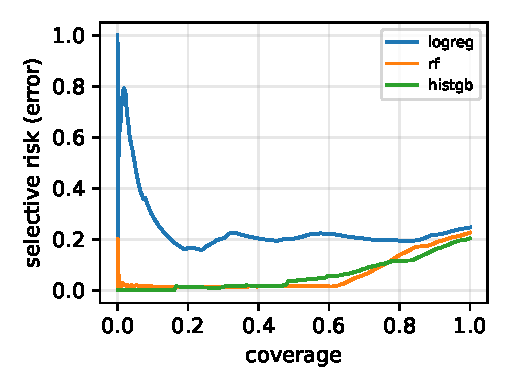
\includegraphics[width=0.82\columnwidth]{figures/risk_coverage.pdf}
\caption{Risk--coverage curves on NSL-KDD. Tree ensembles rank errors well; the linear model does not.}
\label{fig:rc}
\end{figure}

\begin{figure}[t]
\centering
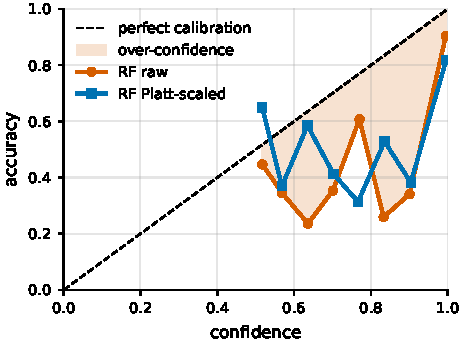
\includegraphics[width=0.82\columnwidth]{figures/reliability_rf.pdf}
\caption{Reliability of the random forest, raw vs.\ Platt-scaled, on the shifted test set.}
\label{fig:rel}
\end{figure}

\subsection{Unknown attacks: collapse and partial cover}\label{sec:openset}
On the built-in novel attacks, detection drops sharply: the random forest flags \PH{rf_det_known} of
\emph{known} attacks but only \PH{rf_det_novel} of novel ones. The controlled family-holdout
(Fig.~\ref{fig:open}) confirms this causally: detection of DoS falls from \PH{det_seen_DoS} to
\PH{det_unseen_DoS} when DoS is unknown, and Probe from \PH{det_seen_Probe} to \PH{det_unseen_Probe}.
Abstention rejects \PH{reject_unseen_DoS} of unknown DoS and \PH{reject_unseen_Probe} of unknown Probe
at 80\% coverage---useful but partial. The R2L family is the sharp limit: detected at only
\PH{det_seen_R2L} even when \emph{seen}, falling to \PH{det_unseen_R2L} when unknown, and abstention
flags just \PH{reject_unseen_R2L} of it. Because R2L traffic statistically resembles benign sessions,
the detector is confidently wrong, and a confidence-based reject option cannot save it.

\begin{figure}[t]
\centering
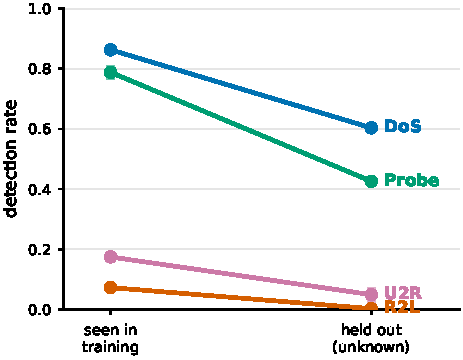
\includegraphics[width=0.82\columnwidth]{figures/openset_detection.pdf}
\caption{Detection rate per family when the family is seen in training vs.\ held out (unknown).}
\label{fig:open}
\end{figure}

\section{Discussion and Limitations}
Selective prediction is a cheap, model-agnostic safety layer: at the cost of deferring a minority of
inputs it materially lowers the error among those acted upon, and it partially flags unknown attacks.
But our results bound the claim. First, the value of abstention is inherited from the confidence
signal, which is good for tree ensembles and poor for the linear model. Second, post-hoc calibration
on source data does not survive distribution shift, so calibrated probabilities should not be trusted
as deployment-time guarantees. Third, and most important operationally, abstention only catches
unknowns that \emph{look} anomalous; attacks that mimic benign traffic (R2L here) are missed
confidently and silently. NSL-KDD is dated and its feature set hand-crafted; confirming these effects
on a modern flow-based corpus is the natural next step.

\section{Conclusion}
On a standard benchmark, off-the-shelf intrusion detectors are over-confident, post-hoc calibration
does not transfer under shift, and a simple reject option lowers selective risk and partially flags
unknown attacks---except those that resemble normal traffic. Selective prediction is worth adding to
ML intrusion detection, provided its confidence signal and its blind spots are measured rather than
assumed.

\section*{Acknowledgment}
The authors used a large language model (Anthropic Claude) to assist with code scaffolding, editing,
and literature search. All experiments, results, and claims were verified by the authors; the AI
system is not an author. Generative-AI use is disclosed per IEEE policy.

\bibliographystyle{IEEEtran}
\bibliography{references}

\end{document}
